\documentclass[../final_report.tex]{subfiles}
\usepackage{subfiles}
\graphicspath{{../../Lab1/plot/}}
\begin{document}

Η συγκεκριμένη άσκηση είναι εισαγωγική με σκοπό την εξοικείωση μας με τα μηχανήματα του cslab στα οποία εκτελούμε τις εργασίες. Για να δοκιμάσουμε την κατανόησή μας, ζητήθηκε να παραλληλοποιήσουμε το Conway’s Game of Life, ένα απλό παιχνίδι το οποίο “παίζεται” πάνω σε ένα ταμπλό (στην δική μας περίπτωση, διαστάσεων N x N). Το παιχνίδι τρέχει για Κ γύρους (χρονικά διαστήματα). Το κάθε σημείο του ταμπλό έχει 2 καταστάσεις, είτε ζωντανό ή νεκρό. Οι 2 κύριοι κανόνες του παιχνιδιού είναι: \newline

1.	Αν ένα ζωντανό σημείο έχει περισσότερους από 3 γείτονες ή λιγότερους από 2, τότε γίνεται νεκρό στον επόμενο γύρο. Αν έχει ακριβώς 2 ή 3, παραμένει ζωντανό. 

2.	Αν ένα νεκρό σημείο έχει ακριβώς 3 γείτονες, γίνεται ζωντανό στον επόμενο γύρο \newline

Τρέχουμε το παραπάνω σενάριο για 1000 γενιές (γύρους) σε πίνακες διαστάσεων 64x64, 1024x1024 και 4096x4096. \newline

Ο κώδικας ο οποίος ζητείται να παραλληλοποιηθεί είναι ο εξής.


\begin{lstlisting}
for ( t = 0 ; t < T ; t++ ) {
        #pragma omp parallel for shared (previous, current) private (i,j,nbrs)
         for ( i = 1 ; i < N-1 ; i++ )
            for ( j = 1 ; j < N-1 ; j++ ) {
                nbrs = previous[i+1][j+1] + previous[i+1][j] + previous[i+1][j-1] \
                       + previous[i][j-1] + previous[i][j+1] \
                       + previous[i-1][j-1] + previous[i-1][j] + previous[i-1][j+1];
                if ( nbrs == 3 || ( previous[i][j]+nbrs ==3 ) )
                    current[i][j]=1;
                else
                    current[i][j]=0;
            }

        #ifdef OUTPUT
        print_to_pgm(current, N, t+1);
        #endif
        //Swap current array with previous array
        swap=current;
        current=previous;
        previous=swap;
    }
\end{lstlisting}



Το πρώτο for-loop, το οποίο είναι η αλλαγή των γενιών, δεν έχει νόημα να παραλληλοποιηθεί αφού χρειαζόμαστε την τιμή της προηγούμενης γενιάς για να υπολογίσουμε τις καταστάσεις των κελιών για την επόμενη γενιά.


Η δική μας προσθήκη στον κώδικα είναι η γραμμή.

\begin{lstlisting}
 #pragma omp parallel for shared (previous, current) private (i,j,nbrs)
\end{lstlisting}


Το συγκεκριμένο compiler directive (pragma) είναι χαρακτηριστικό του OpenMP. Είναι μια “οδηγία” προς τον μεταγλωττιστή η οποία του ζητάει να παραλληλοποιηθούν τα εσωτερικά for-loops με νήματα ορισμένα από ένα environmental variable. Στο συγκεκριμένο directive, επίσης ζητάμε:

1.	Οι δείκτες previous, current να μοιράζονται μεταξύ των νημάτων. Η διάσταση Ν μοιράζεται by default.

2.	Οι μεταβλητές i,j,nbrs να είναι ξεχωριστές για κάθε νήμα.
\newline

Την απόδοση του πολυνηματισμού θα εξετάσουμε με χρήση την μετρική του χρόνου, και κατά συνέπεια, του speedup $S=\frac{T_s}{T_p}$ . \newline

\begin{figure}[H]
    \centering
    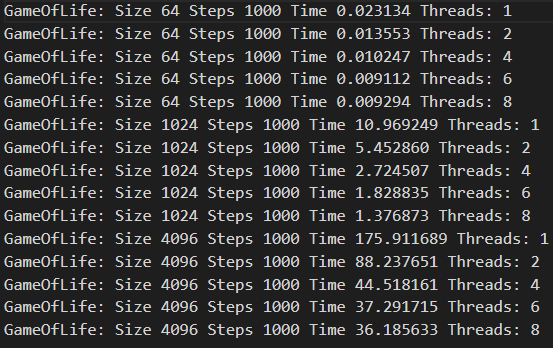
\includegraphics[scale=0.5]{/results.png}
    \caption{Έξοδος Game of Life}
    \label{fig:Έξοδος Game Of Life}
\end{figure}

\begin{figure}[H]
    \centering
    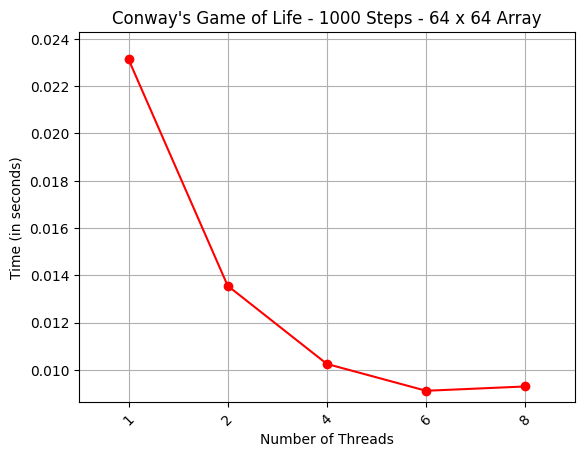
\includegraphics[scale=0.45]{/time_plots/time_64.png}
    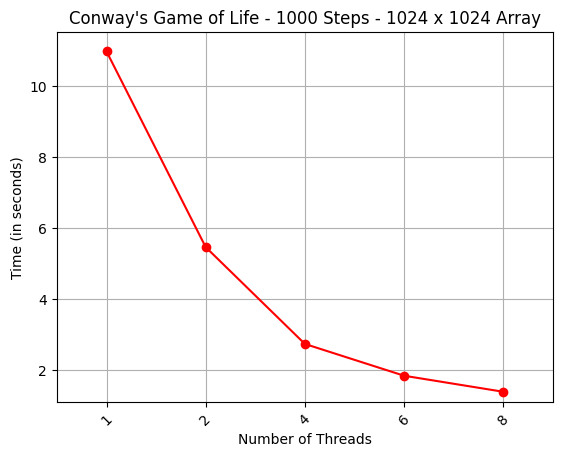
\includegraphics[scale=0.45]{/time_plots/time_1024.png}
    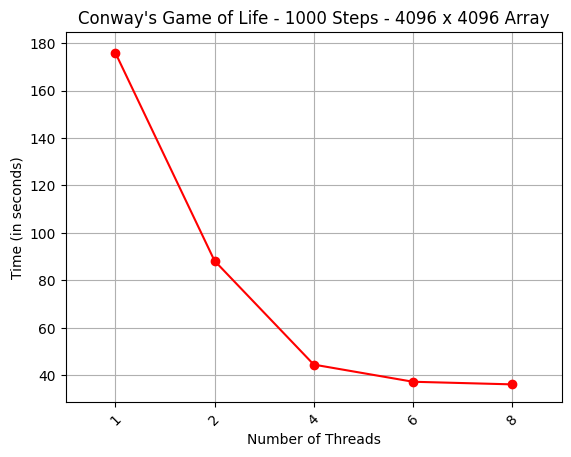
\includegraphics[scale=0.45]{/time_plots/time_4096.png}
    \caption{Χρόνος Εκτέλεσης Game of Life}
    \label{fig:Χρόνος Εκτέλεσης Game Of Life}
\end{figure}

\begin{figure}[H]
    \centering
    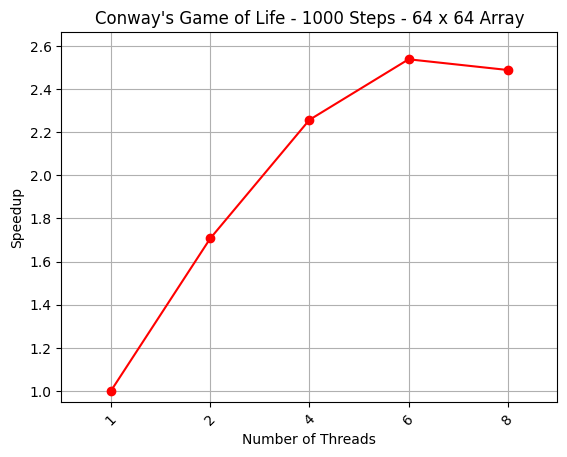
\includegraphics[scale=0.4]{/speedup_plots/speedup_64.png}
    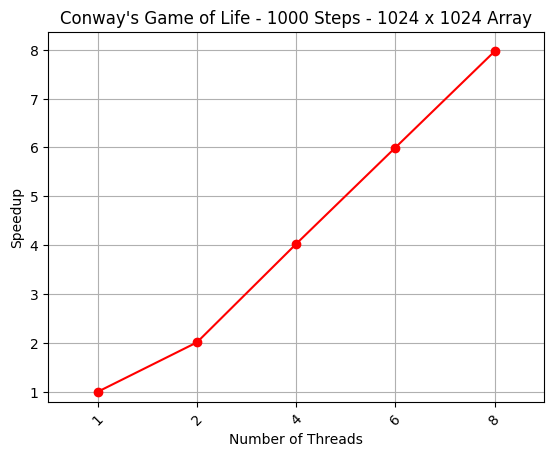
\includegraphics[scale=0.4]{/speedup_plots/speedup_1024.png}
    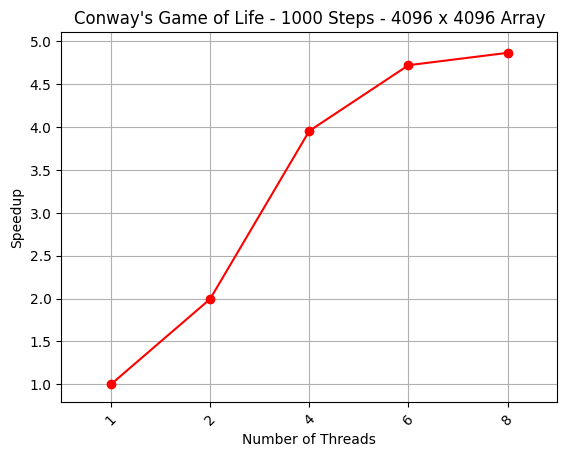
\includegraphics[scale=0.4]{/speedup_plots/speedup_4096.png}
    \caption{Speedup Game of Life}
    \label{fig:Speedup Game Of Life}
\end{figure}

\subsection*{Συμπεράσματα}
\subsubsection*{Για διαστάσεις 64x64}

Παρατηρούμε ότι η μείωση του χρόνου δεν είναι ακριβώς ανάλογη των αριθμών των νημάτων. Από 1 σε 2 νήματα ή από 2 σε 4 νήματα βλέπουμε σημαντική βελτίωση της απόδοσης. Η εναλλαγή από 4 σε 6 νήματα προσφέρει πολύ μικρότερη αύξηση απόδοσης. Τέλος, από 6 σε 8 νήματα παρατηρούμε \textbf{ΑΥΞΗΣΗ} του χρόνου εκτέλεσης (μηδαμινή). 

Η συγκεκριμένη αύξηση οφείλεται στο overhead που υπάρχει με την χρήση πολυνηματισμού σε μια διεργασία (γέννηση νημάτων, επικοινωνία κ.λ.π.). Ο συγκεκριμένος πίνακας είναι τόσο μικρός που η παραλληλοποίησή του περαιτέρω δεν βγάζει νόημα. Αν είχαμε την δυνατότητα να εξετάσουμε μεγαλύτερο αριθμό νημάτων, πολύ πιθανό να βλέπαμε περαιτέρω αύξηση του χρόνου εκτέλεσης
\subsubsection*{Για διαστάσεις 1024x1024}

Παρατηρούμε ότι το speedup τείνει να είναι πλήρως γραμμικό. Ο χρόνος υποδιπλασιάζεται με κάθε διπλασιασμό νημάτων. Το συγκεκριμένο ταμπλό φαίνεται ιδανικό για παραλληλοποίηση. Η επικοινωνία μεταξύ νημάτων δεν περιορίζει την απόδοσή τους
\subsubsection*{Για διαστάσεις 4096x4096}

Στους πρώτους 2 διπλασιασμούς των threads, βλέπουμε γραμμική μείωση του χρόνου (υποδιπλασιασμός) και κατά συνέπεια γραμμική αύξηση του speedup. Η λογική αυτή σταματάει να ισχύει για περαιτέρω αύξηση των νημάτων. Το συγκεκριμένο φαινόμενο δικαιολογείται από την ύπαρξη μεγάλου φόρτου (συμφόρησης) στον διάδρομο μνήμης. Υπάρχει συχνός διαμοιρασμός δεδομένων μεταξύ νημάτων καθώς αυξάνονται οι τιμές που πρέπει να ελεγχθούν για να υπολογιστούν οι γείτονες.

\end{document}